% !TeX root = Auswertung.tex

\subsection{Grundlagen}

Ein Laser Besteht grundlegend aus drei Komponenten, aus dem Lasermedium, einer Pumpquelle und einem Resonator. Das Lasermedium wird mithilfe der Pumpquelle angeregt und emittiert Licht, durch den Resonator wird das verstärkt. Dieser Aufbau hat den Vorteil, dass das Licht monochromatisch ist, mit hoher Intensität und Kohärenz.
\subsection{Zwei Niveau Laser}
\begin{figure}
\centering
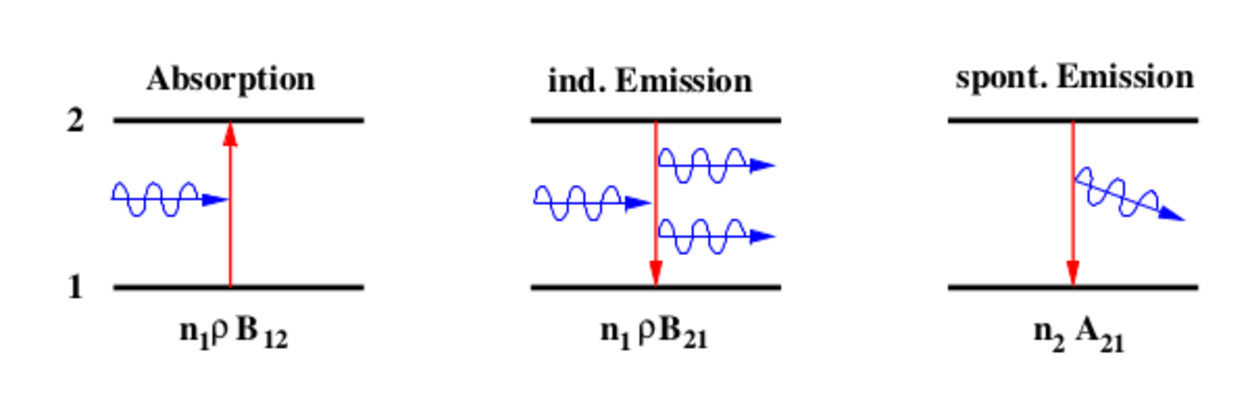
\includegraphics[scale=0.75]{../Grafiken/Emission.pdf}
\caption{Eine Veranschaulichung der Funktionsweise eines zwei Niveau Lasers\cite{V61}}\label{Emission}
\end{figure}
Der einfachste theoretische Laser, ist wenn das Lasermedium  zwei Niveaus besitzt. Die Besetztungszahlen werden mit $n_1$ für das Grundniveau und $n_2$ für den angeregten Zustand bezeichnet. Durch ein Photon mit genügend Energie wird es Absorbiert und System geht in den angeregten Zustand über.\\
Vom angeregten Zustand kann es durch spontane oder induzierten Emission zurück in den Grundzustand zurück. Die Kohärenz wird durch die stimulierten Emission erreicht. Dabei löst ein Photon ein weiteres aus dem System, das dann wieder in den Grundzustand übergeht. Das ausgelöste Photon hat die Selbe Energie, Phase und die Selbe Ausbreitungsrichtung, wie das Photon welches es ausgelöst hat. Wird nun ein Strahlenfeld $\rho$ angelegt, so wird durch Wechselwirkung die Besetzungsdichte $n_2$ durch Emission verringert und durch Absorption erhöht.
Die Änderung der Photonen Anzahl in einem Volumen wird durch
\begin{align*}
\dot{N}_A=n_1 \rho B_{12}\\
\dot{N}_{IE}=n_2\rho B_{21}\\
\dot{N}_{SE}=n_2A_{21}
\end{align*}
gegeben, dabei ist $\dot{N}_A$ die Änderung der Photonen durch Absorption, $\dot{N}_{IE}$ die Änderung der Photonen durch induzierte Emission und $\dot{N}_{SE}$ die Änderung durch Spontane Emission. Die Konstanten $A_{21}$, $B_{12}$ und $B_{21}$ sind die Einsteinkoeffizienten und geben die Übergangswahrscheinlichkeiten an.\\
Unter der Annahme das keine Verluste auftreten, also die Summe von $n_1$ und $n_2$ ist konstant, dann ergeben sich die Ratengleichungen als
\begin{align*}
\frac{dn_1}{dt}=&-n_1 \rho B_{12} + n_2\rho B_{21} + n_2 A_{21}\\
\frac{dn_2}{dt}=&+n_1\rho B_{12} - n_2\rho B_{21} -n_2A_{21}.
\end{align*}
Ein zwei Niveau Laser ist nicht möglich. Wenn beide Zustände gleich viel besetzt sind, ist die Wahrscheinlichkeit das ein Photon durch stimulierte Emission emittiert wird, genauso groß wie das ein Photon absorbiert wird, zusätzlich werden Photonen immer noch durch spontane Emission emittiert.
\subsection{Stabilität eines Lasers}
\begin{figure}[h!]
\centering
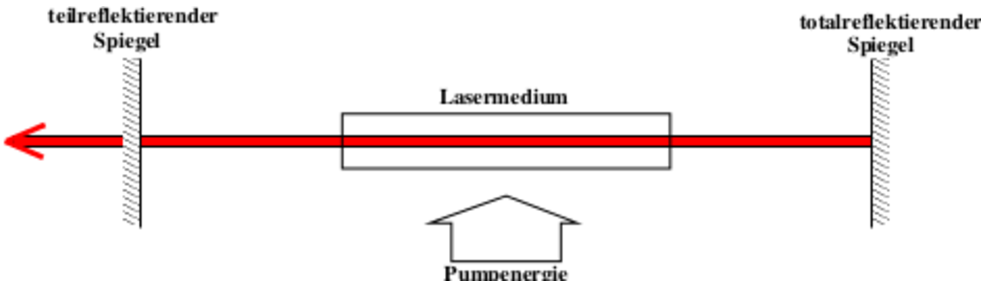
\includegraphics[scale=0.75]{../Grafiken/Laser.pdf}
\caption{Die Skizze eines Lasers\cite{V61}}\label{SkizzeLaser}
\end{figure}
Damit der Strahl des Lasers dauerhaft kohärent bleibt, müssen in den höheren Niveaus mehr besetzt sein als das Grundniveau, dadurch tritt spontane Emission seltener als induzierter Emission auf, dies wird als Besetzungsinversion bezeichnet. Um diesen Zustand zu erzeugen und aufrecht zu erhalten, muss mithilfe der Pumpquelle, dem Lasermedium dauerhaft Energie hinzugefügt werden. Dies geschieht durch Elektronenstöße oder optischer Anregung. Durch einen optischen Resonator wird die Strecke, die der Strahl zur Anregung, durch das Lasermedium zurücklegt Maximiert.\\
Einer der beiden Resonatorspiegel ist teil durchlässig, dadurch wird ein teil des Strahls aus gekoppelt. Die Verluste durch die Resonatorspiegel müssen minimal gehalten werden. Durch konfokale Spiegel deren Brennpunkte aufeinander Fallen, ist dies der Fall.\\
Sind die Verstärkung durch die induzierte Emission größer als die Verluste durch die Resonatorspiegel, dann ist der Resonator stabil. Dann wird
\begin{align}
0\le g_1\cdot g_2 < 1
\end{align}
erfüllt, dabei ist $g_i=1-L/r_i$ und $L$ die Resonatorlänge und $r_i$ der Krümmungsradius des jeweiligen Spiegels. Die Stabilität ist somit nicht nur von dem Typ des Resonators sondern auch von dem Krümmungsradius der Spiegel.
\subsection{TEM-Moden}
Innerhalb des Resonators befinden sich $q$ Wellenlängen die sich longitudinal ausbreiten, weil die Resonatorlänge $L$ um einiges größer ist als die Wellenlänge $\lambda$, $q$ wird auch die longitudinale Mode genannt. Aufgrund von Unebenheiten oder Verkippung des Spiegels entstehen auch transversale Moden $l$ und $q$ die für die $x-$ und $y-$Richtungne stehen. Daraus ergibt sich $TEM_{lpq}$ (transverse electromagnetic Mode) die als Anlehnung an den Hohlleiter verwendet wird. Die Modenzahl $q$ kann meistens Weggelassen werden weil sie von keiner Bedeutung ist. In den meisten Resonatoren werden nur wenige Moden isoliert und verstärkt.\\
%%%%%%%%%%%%%%%%%%%%%%%%%Wenn Verteilung hier Einfügen%%%%%%%%%%%%%%%%%%%%%%%%%%%%%%%%%%%%%%%%%
Die Grundmode $TEM_{00}$ ist die Mode mit der höchsten Symmetrie und den wenigsten Verlusten. Die Intensität von der Mode wird durch die Gaußverteilung beschrieben.
\begin{align}
I(r)=I_0\exp\left(\frac{-2r^2}{\omega^2}\right)
\end{align}
Hier ist $I_0$ die Maximalintensität, $r$ der Abstand zur optischen Achse und $\omega$ der Strahlenradius. Der Strahlenradius lässt sich durch
\begin{align}
\omega(z)=\omega_0 \sqrt{1+\left(\frac{\theta z}{\omega_0}\right)^2}
\end{align}
beschreiben, dabei ist $\omega_0$ der minimale Strahltaille und $z$ der Abstand und $\theta$ die Strahlendivergenz, wie durch die Gaußsche Strahlenoptik beschrieben.
\subsection{Der HeNe-Laser}
Der HeNe-Laser gehört zu den Gaslasern und das Gemisch aus Helium und Neon hat ein Verhältnis von 5 zu 1 und innerhalb der Laserrohrs befindet sich ein Druck von 1 Torr.Dabei fungiert Helium als Pumpquelle und Neon als Lasermedium. Durch elektrische Entladung wird das Helium in den Angeregten zustand versetzt und gibt die Anregungsenergie durch Stöße zweiter Ordnung an das Neon ab, dadurch kann Besetzungsinversion auftreten. Der Laser besitzt die intensivste Wellenlänge bei $\lambda=$632,8nm.